%\RequirePackage[l2tabu, orthodox]{nag}
\documentclass[12pt]{beamer}
\graphicspath{{Imagenes/}{../Imagenes/}}
\usepackage[utf8]{inputenc}
\usepackage[spanish]{babel}
\usepackage[autostyle,spanish=mexican]{csquotes}
\usepackage{hyperref}
\hypersetup{
  colorlinks=true,
  linkcolor=blue,          % color of internal links (change box color with linkbordercolor)
  citecolor=green,        % color of links to bibliography
  filecolor=magenta,      % color of file links
  urlcolor=cyan,           % color of external links
  linkbordercolor={0 0 1}
}
\usepackage{amsmath}
\usepackage{amsthm}
\usepackage{multicol}
\usepackage{graphicx}
\usepackage{physics}
\usepackage{tabulary}
\usepackage{booktabs}
\usepackage[outdir=./]{epstopdf}
%\usepackage{epstopdf}
\usepackage{media9}
\usepackage{multimedia}
\usepackage[binary-units=true]{siunitx}
\usepackage{standalone}
\usepackage{longtable}
\usepackage{bigints}
\usepackage[font=footnotesize,textfont=it]{caption}
%\usepackage{enumitem}
\usepackage{tikz}
\usetikzlibrary{mindmap}
\usepackage[siunitx]{circuitikz}
\usetikzlibrary{arrows, patterns, shapes, decorations.markings, decorations.pathmorphing}
\usetikzlibrary{matrix,positioning}
\tikzstyle{every picture}+=[remember picture,baseline]
\usepackage{color}
\usepackage{alltt}
\usepackage{verbatim}
\usepackage{colortbl}
\usepackage{fancyvrb}
\usepackage[os=win]{menukeys}
\usepackage{pifont}
\usepackage[sfdefault]{roboto}  %% Option 'sfdefault' only if the base font of the document is to be sans serif
%\usepackage[T1]{fontenc}
\setcounter{secnumdepth}{3}
\setcounter{tocdepth}{3}
\DeclareGraphicsExtensions{.pdf,.png,.jpg}
\renewcommand {\arraystretch}{1.5}
\definecolor{ao}{rgb}{0.0, 0.5, 0.0}
\definecolor{bisque}{rgb}{1.0, 0.89, 0.77}
\definecolor{amber}{rgb}{1.0, 0.75, 0.0}
\definecolor{armygreen}{rgb}{0.29, 0.33, 0.13}
\definecolor{alizarin}{rgb}{0.82, 0.1, 0.26}
\definecolor{cadetblue}{rgb}{0.37, 0.62, 0.63}
\newcommand*{\TitleParbox}[1]{\parbox[c]{6cm}{\raggedright #1}}%
\newcommand{\python}{\texttt{python}}
\newcommand{\textoazul}[1]{\textcolor{blue}{#1}}
\newcommand{\azulfuerte}[1]{\textcolor{blue}{\textbf{#1}}}
\newcommand{\funcionazul}[1]{\textcolor{blue}{\textbf{\texttt{#1}}}}
%\normalfont
\usepackage{ccfonts}% http://ctan.org/pkg/{ccfonts}
\usepackage[T1]{fontenc}% http://ctan.or/pkg/fontenc
\renewcommand{\rmdefault}{cmr}% cmr = Computer Modern Roman
\usefonttheme[onlymath]{serif}
\linespread{1.3}
\newcounter{saveenumi}
\newcommand{\seti}{\setcounter{saveenumi}{\value{enumi}}}
\newcommand{\conti}{\setcounter{enumi}{\value{saveenumi}}}
\newcommand{\tikzmark}[1]{\tikz[remember picture] \node[coordinate] (#1) {#1};}

\usepackage{scalerel}[2016-12-29]
\def\stretchint#1{\vcenter{\hbox{\stretchto[440]{\displaystyle\int}{#1}}}}
\def\scaleint#1{\vcenter{\hbox{\scaleto[3ex]{\displaystyle\int}{#1}}}}
\def\bs{\mkern-12mu}

\newtheorem{teo}{}[section]
\usepackage{blkarray}

%reduce el tamaño de letra de la etiqueta equations
\makeatletter
\def\maketag@@@#1{\hbox{\m@th\normalfont\small#1}}
\makeatother

%se usa para la x en itemize
\newcommand{\xmark}{\text{\ding{55}}}

%\AtBeginDocument{\setlength{\tymin}{1em}}


\definecolor{myblue}{rgb}{.8, .8, 1}

\usepackage{amsmath}
\usepackage{empheq}

\newlength\mytemplen
\newsavebox\mytempbox

\makeatletter
\newcommand\mybluebox{%
    \@ifnextchar[%]
       {\@mybluebox}%
       {\@mybluebox[0pt]}}

\def\@mybluebox[#1]{%
    \@ifnextchar[%]
       {\@@mybluebox[#1]}%
       {\@@mybluebox[#1][0pt]}}

\def\@@mybluebox[#1][#2]#3{
    \sbox\mytempbox{#3}%
    \mytemplen\ht\mytempbox
    \advance\mytemplen #1\relax
    \ht\mytempbox\mytemplen
    \mytemplen\dp\mytempbox
    \advance\mytemplen #2\relax
    \dp\mytempbox\mytemplen
    \colorbox{myblue}{\hspace{1em}\usebox{\mytempbox}\hspace{1em}}}

\makeatother



\usepackage{courier}
\usepackage{listingsutf8}
\usepackage{listings}
\usepackage{xcolor}
\usepackage{textcomp}
\usepackage{color}
\definecolor{deepblue}{rgb}{0,0,0.5}
\definecolor{brown}{rgb}{0.59, 0.29, 0.0}
\definecolor{OliveGreen}{rgb}{0,0.25,0}
% \usepackage{minted}

\DeclareCaptionFont{white}{\color{white}}
\DeclareCaptionFormat{listing}{\colorbox{gray}{\parbox{0.98\textwidth}{#1#2#3}}}
\captionsetup[lstlisting]{format=listing,labelfont=white,textfont=white}
\renewcommand{\lstlistingname}{Código}


\definecolor{Code}{rgb}{0,0,0}
\definecolor{Keywords}{rgb}{255,0,0}
\definecolor{Strings}{rgb}{255,0,255}
\definecolor{Comments}{rgb}{0,0,255}
\definecolor{Numbers}{rgb}{255,128,0}

\makeatletter

\newif\iffirstchar\firstchartrue
\newif\ifstartedbyadigit
\newif\ifprecededbyequalsign

\newcommand\processletter
{%
  \ifnum\lst@mode=\lst@Pmode%
    \iffirstchar%
        \global\startedbyadigitfalse%
      \fi
      \global\firstcharfalse%
    \fi
}

\newcommand\processdigit
{%
  \ifnum\lst@mode=\lst@Pmode%
      \iffirstchar%
        \global\startedbyadigittrue%
      \fi
      \global\firstcharfalse%
  \fi
}

\lst@AddToHook{OutputOther}%
{%
  \lst@IfLastOtherOneOf{=}
    {\global\precededbyequalsigntrue}
    {}%
}

\lst@AddToHook{Output}%
{%
  \ifprecededbyequalsign%
      \ifstartedbyadigit%
        \def\lst@thestyle{\color{orange}}%
      \fi
    \fi
  \global\firstchartrue%
  \global\startedbyadigitfalse%
  \global\precededbyequalsignfalse%
}

\lstset{ 
language=Python,                % choose the language of the code
basicstyle=\footnotesize\ttfamily,       % the size of the fonts that are used for the code
numbers=left,                   % where to put the line-numbers
numberstyle=\scriptsize,      % the size of the fonts that are used for the line-numbers
stepnumber=1,                   % the step between two line-numbers. If it is 1 each line will be numbered
numbersep=5pt,                  % how far the line-numbers are from the code
backgroundcolor=\color{white},  % choose the background color. You must add \usepackage{color}
showspaces=false,               % show spaces adding particular underscores
showstringspaces=false,         % underline spaces within strings
showtabs=false,                 % show tabs within strings adding particular underscores
frame=single,   		% adds a frame around the code
tabsize=2,  		% sets default tabsize to 2 spaces
captionpos=t,   		% sets the caption-position to bottom
breaklines=true,    	% sets automatic line breaking
breakatwhitespace=false,    % sets if automatic breaks should only happen at whitespace
escapeinside={| |},  % if you want to add a comment within your code
stringstyle =\color{OliveGreen},
otherkeywords={as, np.array, np.concatenate, np.linspace, linspace, interpolate.interp1d, kind, plt.plot, .copy, np.arange, np.cos, np.pi, lw, ls, label, splrep, splev, plt.legend, loc, plt.title, plt.ylim, plt.show, sign, math.ceil, math.log, np.sqrt, np.exp, np.zeros, plt.xlabel, plt.ylabel, plt.xlim, np.identity, random, np.dot, np.outer, np.diagonal },             % Add keywords here
keywordstyle = \color{blue},
commentstyle = \color{darkcerulean},
identifierstyle = \color{black},
literate=%
         {á}{{\'a}}1
         {é}{{\'e}}1
         {í}{{\'i}}1
         {ó}{{\'o}}1
         {ú}{{\'u}}1
%
%keywordstyle=\ttb\color{deepblue}
%fancyvrb = true,
}

\lstdefinestyle{FormattedNumber}{%
    literate={0}{{\textcolor{red}{0}}}{1}%
             {1}{{\textcolor{red}{1}}}{1}%
             {2}{{\textcolor{red}{2}}}{1}%
             {3}{{\textcolor{red}{3}}}{1}%
             {4}{{\textcolor{red}{4}}}{1}%
             {5}{{\textcolor{red}{5}}}{1}%
             {6}{{\textcolor{red}{6}}}{1}%
             {7}{{\textcolor{red}{7}}}{1}%
             {8}{{\textcolor{red}{8}}}{1}%
             {9}{{\textcolor{red}{9}}}{1}%
             {.0}{{\textcolor{red}{.0}}}{2}% Following is to ensure that only periods
             {.1}{{\textcolor{red}{.1}}}{2}% followed by a digit are changed.
             {.2}{{\textcolor{red}{.2}}}{2}%
             {.3}{{\textcolor{red}{.3}}}{2}%
             {.4}{{\textcolor{red}{.4}}}{2}%
             {.5}{{\textcolor{red}{.5}}}{2}%
             {.6}{{\textcolor{red}{.6}}}{2}%
             {.7}{{\textcolor{red}{.7}}}{2}%
             {.8}{{\textcolor{red}{.8}}}{2}%
             {.9}{{\textcolor{red}{.9}}}{2}%
             {\ }{{ }}{1}% handle the space
         ,%
          %mathescape=true
          escapeinside={__}
          }



%Se usa la plantilla Warsaw modificada con spruce
\mode<presentation>
{
  \usetheme{Warsaw}
  \setbeamertemplate{headline}{}
  \useoutertheme{default}
  \usecolortheme{seahorse}
  \setbeamercovered{invisible}
}
% \AtBeginSection[]
% {
% \begin{frame}<beamer>{Contenido}
% \normalfont\mdseries
% \tableofcontents[currentsection]
% \end{frame}
%}
\makeatletter
\setbeamertemplate{footline}
{
  \leavevmode%
  \hbox{%
  \begin{beamercolorbox}[wd=.333333\paperwidth,ht=2.25ex,dp=1ex,center]{author in head/foot}%
    \usebeamerfont{author in head/foot} \textcolor{purple}{\insertsection}
  \end{beamercolorbox}}%
  \begin{beamercolorbox}[wd=.333333\paperwidth,ht=2.25ex,dp=1ex,center]{title in head/foot}%
    \usebeamerfont{title in head/foot}\insertsubsection
  \end{beamercolorbox}%
  \begin{beamercolorbox}[wd=.333333\paperwidth,ht=2.25ex,dp=1ex,right]{date in head/foot}%
    \usebeamerfont{date in head/foot}\insertshortdate{}\hspace*{2em}
    \insertframenumber{} / \inserttotalframenumber\hspace*{2ex} 
  \end{beamercolorbox}}%
  \vskip0pt%
\makeatother
\setbeamertemplate{navigation symbols}{}
\normalfont
\usepackage{ccfonts}% http://ctan.org/pkg/{ccfonts}
\usepackage[T1]{fontenc}% http://ctan.or/pkg/fontenc
\renewcommand{\rmdefault}{cmr}% cmr = Computer Modern Roman
\linespread{1.3}
\title{\textcolor{black}{Métodos de Monte Carlo - 3}}
\subtitle{Curso de Física Computacional}
\author[]{M. en C. Gustavo Contreras Mayén}
\setbeamercolor{background canvas}{bg=white} %white = default
\setbeamertemplate{caption}[numbered]
\setbeamercolor{caption name}{fg=structure!20!blue}
\setbeamercolor{section in toc}{fg=blue}
\setbeamercolor{subsection in toc}{fg=blue!85}
\setbeamercolor{section number projected}{bg=black,fg=yellow}
\setbeamertemplate{subsection in toc}{%
  \hspace{1.2em}{\color{orange}\rule[0.3ex]{3pt}{3pt}}~\inserttocsubsection\par}
\setbeamercolor{framesubtitle}{fg=blue}
\beamertemplatenavigationsymbolsempty
\begin{document}
\newcommand{\localtextbulletone}{\textcolor{gray}{\raisebox{.45ex}{\rule{.6ex}{.6ex}}}}
\maketitle
\fontsize{14}{14}\selectfont
\spanishdecimal{.}
\section{Caminatas aleatorias}
\frame{\tableofcontents[currentsection, hideothersubsections]}
\subsection{Definición}
\begin{frame}
\frametitle{Definición}
Las \emph{caminatas} aleatorias son trayectorias en donde se dan pasos sucesivos en direcciones aleatorias.
\\
\bigskip
\pause
Surgen en la mecánica estadística: como sumas parciales de cantidades que varían, como trayectorias de partículas sometidas a colisiones repetidas, y como las estructuras largas de sistemas vinculados como los polímeros.
\end{frame}
\subsection*{Comportamiento emergente}
\begin{frame}
\frametitle{Comportamiento emergente}
Presentan dos clases de comportamiento emergente:
\setbeamercolor{item projected}{bg=red!70!black,fg=white}
\setbeamertemplate{enumerate items}[circle]
\begin{enumerate}[<+->]
\item En primer lugar, una caminata aleatoria individual, después de un gran número de pasos, se convierte en invariante fractal o de escala.
\item En segundo lugar, el punto final de la caminata aleatoria tiene una distribución de probabilidad que obedece a una ley continua simple: la ecuación de difusión.
\end{enumerate}
\end{frame}
\begin{frame}
\frametitle{Comportamiento emergente}
Ambos comportamientos son en gran parte independientes de los detalles microscópicos de la caminata, son universales.
\\
\bigskip
Las caminatas aleatorias ilustran perfectamente muchos de los temas y métodos de la mecánica estadística.
\end{frame}
\section{Universalidad e invarianza de escala}
\frame{\tableofcontents[currentsection, hideothersubsections]}
\subsection{Cantidades que varían}
\begin{frame}
\frametitle{Universalidad e invarianza de escala}
La mecánica estadística suele exigir sumas o promedios de una serie de cantidades que varían:\[\ s_{N} = \sum_{i = 1}^{N} \ell_{i}  \]
\end{frame}
\begin{frame}
\frametitle{Universalidad e invarianza de escala}
La energía de un material es la suma sobre las energías de las moléculas que componen el material.
\end{frame}
\begin{frame}
\frametitle{Universalidad e invarianza de escala}
Tu calificación final de física computacional es la suma de los puntos tanto de tareas como de exámenes. Ahora imagínate sumando cada término a la vez.
\\
\bigskip
La trayectoria $s_{1}, s_{2}, \ldots$ forma un ejemplo de una caminata aleatoria unidimensional.
\end{frame}
\section{Ejemplos de caminatas aleatorias}
\frame{\tableofcontents[currentsection, hideothersubsections]}
\subsection{Lanzamiento de monedas}
\begin{frame}
\frametitle{Lanzamiento de monedas}
Considera el lanzar una moneda y registrar la diferencia $s_{N}$ entre el número de águilas y soles encontradas.
\\
\bigskip
Cada lanzamiento de moneda aporta $\ell_{i} = \pm 1$ del total.
\pause
\end{frame}
\begin{frame}
\frametitle{Lanzamiento de monedas}
¿Qué tan grande será la suma
\[ s_{N} = \sum_{i = 1}^{N} \; \ell_{i} = \mbox{ águilas - soles} \]
luego de $N$ lanzamientos?
\end{frame}
\begin{frame}
\frametitle{Lanzamiento de monedas}
El promedio de $s_{N}$ no es una buena medida para la suma, porque es cero (son igualmente probables tanto pasos positivos, como negativos).
\end{frame}
\begin{frame}
\frametitle{Lanzamiento de monedas}
Podemos medir el valor absoluto promedio $\left\langle \vert s_{N} \vert \right\rangle$, pero resulta que una distancia característica más agradable es la raíz media cuadrática (RMS) de la suma 
\[ \sqrt{ \left\langle s_{N}^{2} \right\rangle } \]
\end{frame}
\begin{frame}
\frametitle{Lanzamiento de monedas}
Luego del primer lanzamiento de la moneda, el cuadrado de la media es
\begin{equation}
\left\langle s_{1}^{2} \right\rangle = 1 = \dfrac{1}{2} \: (-1)^{2} + \dfrac{1}{2} \: (1)^{2}
\label{eq:ecuacion_02_01}
%Entropy Ordenr Parameters Complexity
\end{equation}
\pause
Luego del segundo y tercer lanzamiento de la moneda
\fontsize{12}{12}\selectfont
\begin{align}
\begin{aligned}
\left\langle s_{2}^{2} \right\rangle &= 2 = \dfrac{1}{4} \: (-2)^{2} + \dfrac{1}{2} \: (0)^{2} + \dfrac{1}{4} \: (2)^{2} \\
\left\langle s_{3}^{2} \right\rangle &= 3 = \dfrac{1}{8} \: (-3)^{2} + \dfrac{3}{8} \: (-1)^{2} + \dfrac{3}{8} \: (1)^{2} + \dfrac{1}{8} \: (3)^{2}
\end{aligned}
\label{eq:ecuacion_02_02}
\end{align}
\end{frame}
\begin{frame}
\frametitle{Lanzamiento de monedas}
Por ejemplo, la probabilidad de tener dos águilas en tres lanzamientos es tres de ocho: AAS, SAS y SSS.
\\
\bigskip
Sin usar la computadora, ¿cuál es el valor de $\left\langle s_{7}^{2} \right\rangle$?
\end{frame}
\begin{frame}
\frametitle{¿Patrón de lanzamientos?}
¿Este patrón continua con los siguientes lanzamientos?
\\
\bigskip
Veamos la RMS en $N$ pasos en términos de la misma RMS después de $N -1$ pasos, más el último paso.
\end{frame}
\begin{frame}
\frametitle{¿Patrón de lanzamientos?}
Debido a que el promedio de la suma es la suma del promedio, encontramos
\fontsize{12}{12}\selectfont
\begin{equation}
\left\langle s_{N}^{2} \right\rangle = \left\langle (s_{N - 1}^{2} + \ell_{N})^{2} \right\rangle = \left\langle s_{N - 1}^{2} \right\rangle + 2 \: \left\langle s_{N - 1} \: \ell_{N} \right\rangle + \left\langle \ell_{N}^{2} \right\rangle
\label{eq:ecuacion_02_03}
\end{equation}
\fontsize{14}{14}\selectfont
Ahora, $\ell_{N}$ es $\pm 1$ con igual probabilidad, independientemente de lo que ocurrió antes (y por tanto independiente de $s_{N - 1}$).
\end{frame}
\begin{frame}
\frametitle{¿Patrón de lanzamientos?}
Así
\[ \left\langle s_{N - 1} \: \ell_{N} \right\rangle = \dfrac{1}{2} \: s_{N - 1} \: (+1) + \dfrac{1}{2} \: s_{N - 1} \: (-1) = 0 \]
\pause
Y como sabemos que $\ell_{N}^{2} = 1$ resulta
\fontsize{12}{12}\selectfont
\begin{equation}
\left\langle s_{N}^{2} \right\rangle = \left\langle s_{N - 1}^{2} \right\rangle + 2 \: \left\langle s_{N - 1} \ell_{N} \right\rangle + \left\langle \ell_{N}^{2} \right\rangle = \left\langle s_{N - 1}^{2} \right\rangle + 1
\label{eq:ecuacion_02_04}
\end{equation}
\end{frame}
\begin{frame}
\frametitle{¿Patrón de lanzamientos?}
Si suponemos que
\[ \left\langle s_{N - 1}^{2} \right\rangle = N - 1 \]
hemos demostrado por inducción sobre $N$  que
\[ \left\langle s_{N}^{2} \right\rangle = N \]
\end{frame}
\begin{frame}
De aquí que la raíz cuadrada de la media cuadrada (RMS) de (águilas - soles) es igual a la raíz cuadrada del número de lanzamientos de la moneda
\begin{equation}
\sigma_{s} = \sqrt{\left\langle s_{N}^{2} \right\rangle} = \sqrt{N}
\label{eq:ecuacion_05}
\end{equation}
\end{frame}
\subsection*{Naturaleza de las caminatas aleatorias}
\begin{frame}
\frametitle{Naturaleza de las caminatas aleatorias}
Las caminatas aleatorias también se pueden ver como trayectorias de colisiones sucesivas o giros aleatorios.
\end{frame}
\subsection{Una molécula de perfume}
\begin{frame}
\frametitle{Una molécula de perfume}
Por ejemplo, la trayectoria de una molécula de perfume en una muestra de aire.
\\
\bigskip
Dado que el aire es diluido y las interacciones son de corto alcance, la molécula viajará básicamente en línea recta, con cambios bruscos de velocidad durante pocas colisiones.
\end{frame}
\begin{frame}
\frametitle{Una molécula de perfume}
Después de algunas colisiones sustanciales, la velocidad de la molécula no estará correlacionada con su velocidad original.
\\
\bigskip
La trayectoria que toma la molécula será una caminata irregular, aleatoria en tres dimensiones.
\end{frame}
\begin{frame}
\frametitle{Una molécula de perfume}
La caminata aleatoria de una molécula de perfume involucra direcciones, velocidades aleatorias y pasos, todos ellos aleatorios.
\\
\bigskip
Es más conveniente estudiar los pasos a intervalos de tiempo regulares, por lo que consideraremos el \emph{problema clásico del borracho}.
\end{frame}
\subsection{El problema del borracho}
\begin{frame}
\frametitle{El problema del borracho}
Se supone que un borracho comienza a moverse a partir de un poste en $x = y = 0$.
\\
\bigskip
Hace pasos $\ell_{N}$ cada uno de longitud $L$, en intervalos regulares de tiempo.
\end{frame}
\begin{frame}
\frametitle{No hagan esto en casa!!}
\begin{figure}
	\centering
	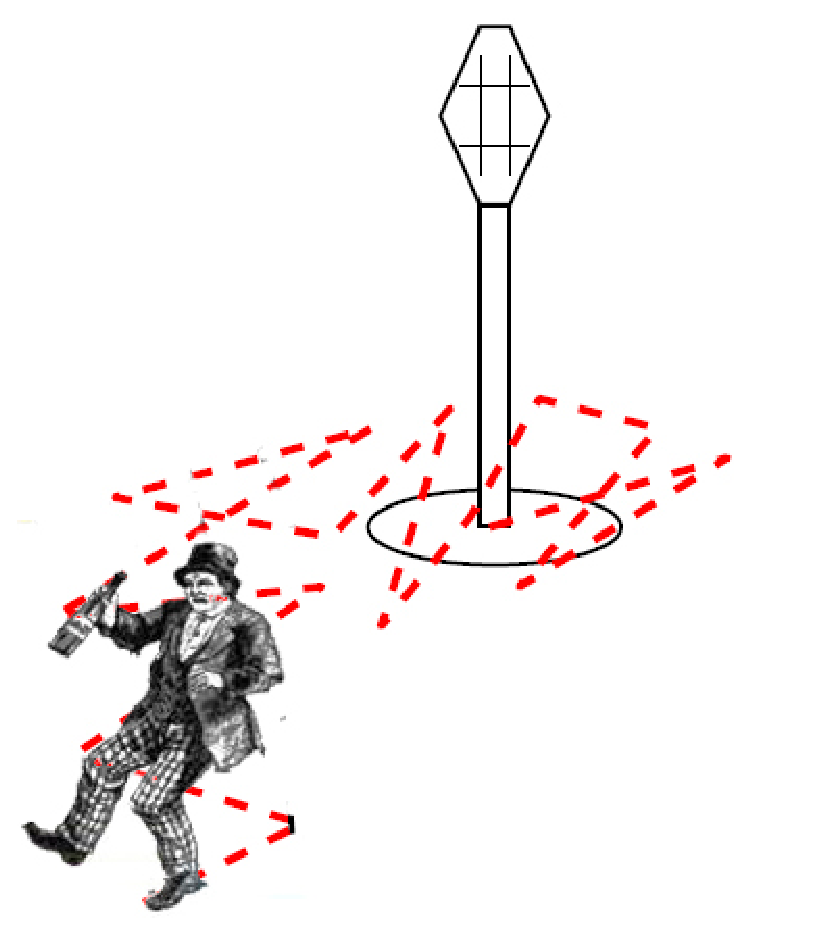
\includegraphics[scale=0.35]{Imagenes/Borracho_03.eps}
	\caption{Ejemplo de un borracho caminando por la calle.}
\end{figure}
\end{frame}
\begin{frame}
\frametitle{El problema del borracho}
Como el amigo está borracho, los pasos que da, están en direcciones completamente aleatorias, cada uno de los pasos no está correlacionado con los pasos anteriores.
\end{frame}
\begin{frame}
\frametitle{El problema del borracho}
Esta falta de correlación indica que el promedio del producto punto entre dos pasos $\ell_{m}$ y $\ell_{n}$ es cero, ya que todos los ángulos relativos $\theta$ entre las dos direcciones son igualmente probables
\[ \left\langle \ell_{m} \cdot \ell_{n} \right\rangle = L^{2} \left\langle \cos \theta \right\rangle = 0 \]
\end{frame}
\begin{frame}
\frametitle{El problema del borracho}
Esto implica que el producto de $\ell_{N}$ con $s_{N - 1} = \sum_{m = 1}^{N - 1} \: \ell_{m}$ es cero.
\\
\bigskip
Usemos esto para nuevamente recurrir a la inducción:
\end{frame}
\begin{frame}
\frametitle{El problema del borracho}
\begin{align}
\begin{aligned}
\left\langle s_{N}^{2} \right\rangle &= \left\langle (s_{N - 1} + \ell_{N})^{2} \right\rangle \\
&=  \left\langle s_{N -1}^{2} \right\rangle + \left\langle 2 \: s_{N - 1} \cdot \ell_{N} \right\rangle + \left\langle \ell_{N}^{2} \right\rangle \\
&= \left\langle s_{N - 1}^{2} \right\rangle + L^{2} \\
&= N \; L^{2}
\end{aligned}
\label{eq:ecuacion_02_06}
\end{align}
\pause
así que la raíz media cuadrática de la distancia recorrida es $\sqrt{N} \: L$.
\end{frame}
\subsection*{Invariancia de escala}
\begin{frame}
\frametitle{Invariancia de escala}
Con $N$ pasos, ¿qué tipo de trayectoria tendríamos con una longitud de $\sqrt{N}$?
\\
\bigskip
\pause
Las caminatas aleatorias forman trayectorias que parecen irregulares y revueltas. 
\\
\bigskip
De hecho, son tan irregulares que si hacemos un zoom en una de ellas, la ventana que veremos se ve tan irregular.
\end{frame}
\begin{frame}[plain]
\frametitle{Ejemplo de una caminata aleatoria}
\framesubtitle{La longitud de esta caminata es de 32000 pasos}
\begin{figure}
	\centering
	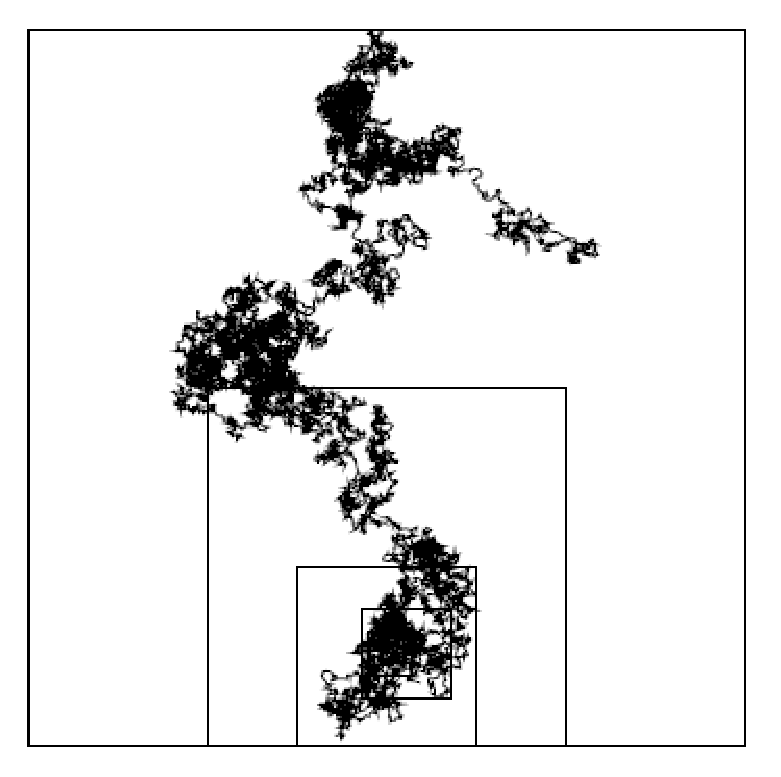
\includegraphics[scale=0.5]{Imagenes/caminataAleatoria_01.eps}
	\caption{Hacemos un zoom a una cuarta parte de la imagen.}
\end{figure}
\end{frame}
\begin{frame}
\frametitle{Cambio de escala}
\begin{figure}
	\centering
	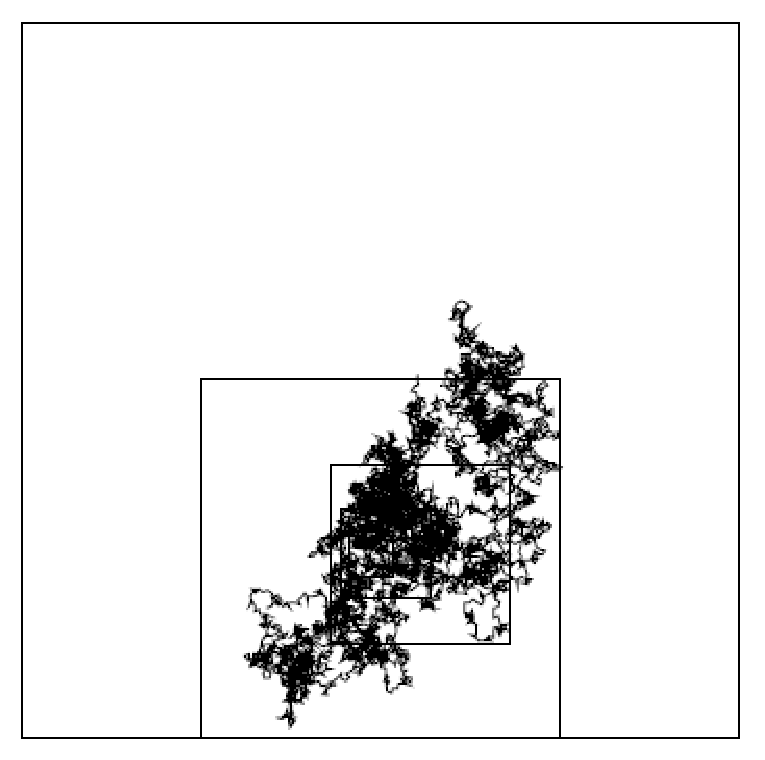
\includegraphics[scale=0.5]{Imagenes/caminataAleatoria_02.eps}
	\caption{La caminata aleatoria de longitud $N/4$, se asemeja a la anterior de longitud $N$.}
\end{figure}
\end{frame}
\begin{frame}
\frametitle{Cambio de escala}
\begin{figure}
	\centering
	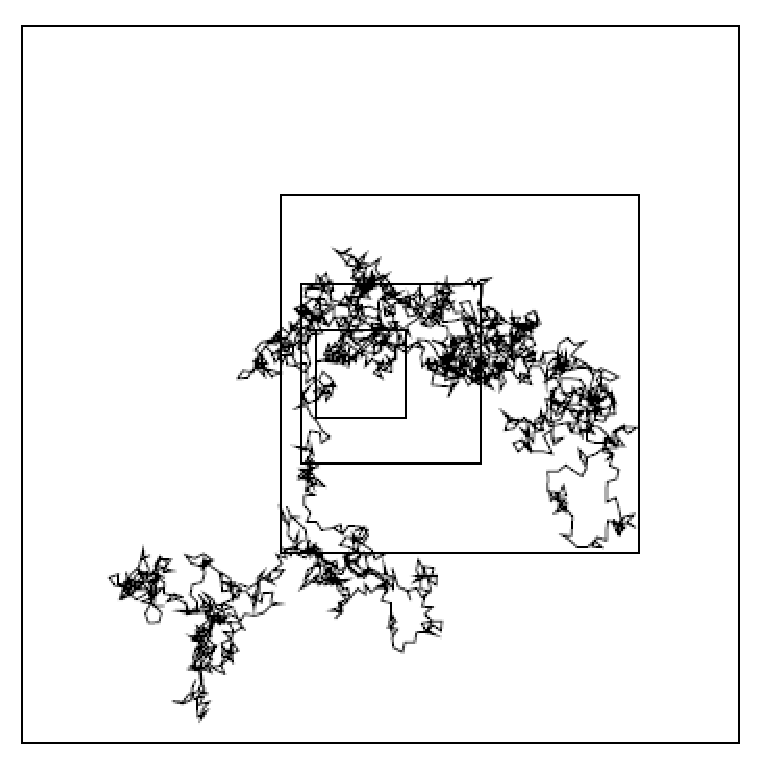
\includegraphics[scale=0.5]{Imagenes/caminataAleatoria_03.eps}
	\caption{Caminata aleatoria de longitud $N/16$.}
\end{figure}
\end{frame}
\begin{frame}
\frametitle{Cambio de escala}
\begin{figure}
	\centering
	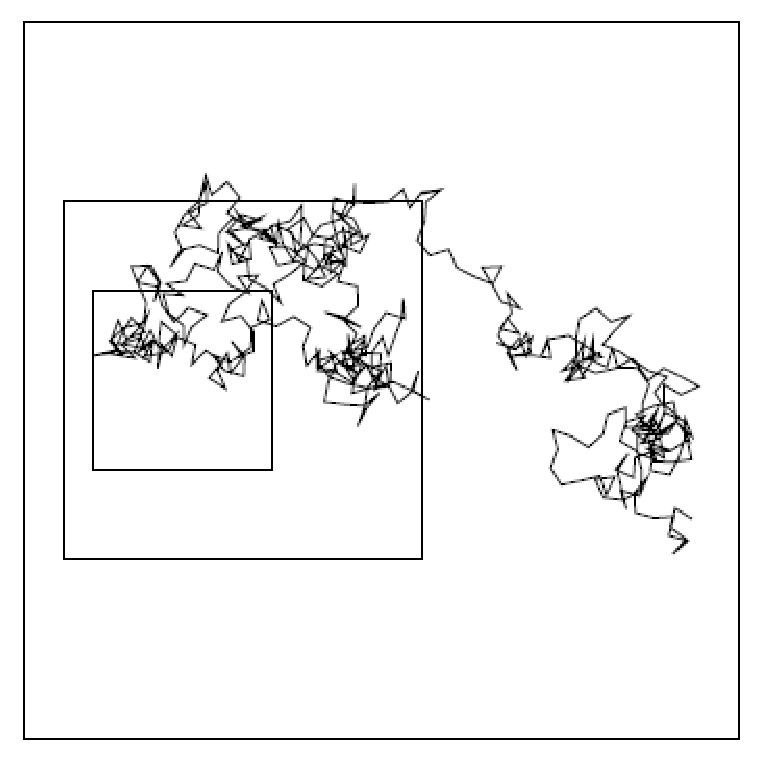
\includegraphics[scale=0.5]{Imagenes/caminataAleatoria_04.eps}
	\caption{Seguimos haciendo zoom a la caminata aleatoria.}
\end{figure}
\end{frame}
\begin{frame}
\frametitle{Cambio de escala}
\begin{figure}
	\centering
	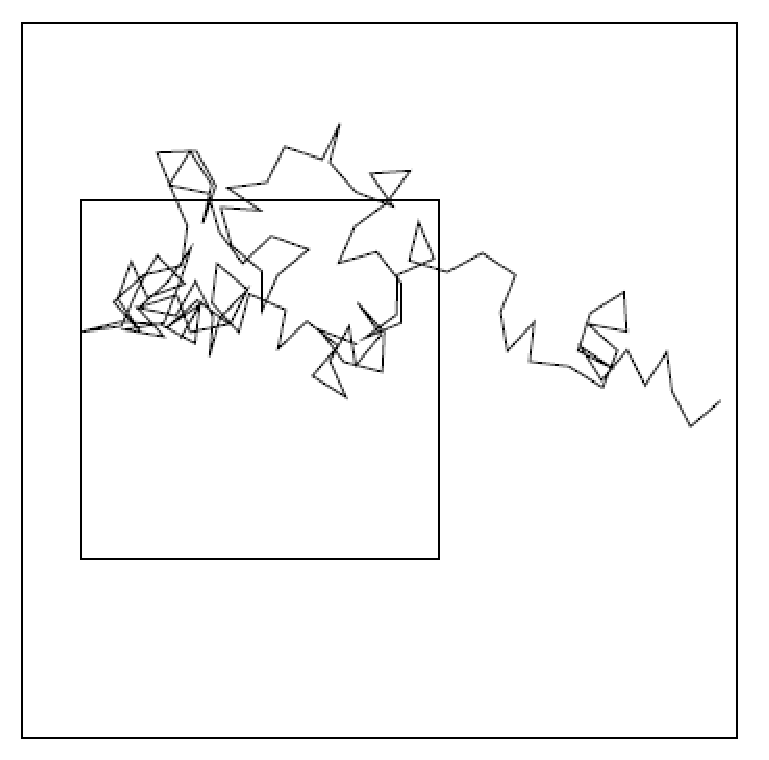
\includegraphics[scale=0.5]{Imagenes/caminataAleatoria_05.eps}
	\caption{Ya se distinguen los pasos de la caminata.}
\end{figure}
\end{frame}
\begin{frame}
\frametitle{Cambio de escala}
\begin{figure}
	\centering
	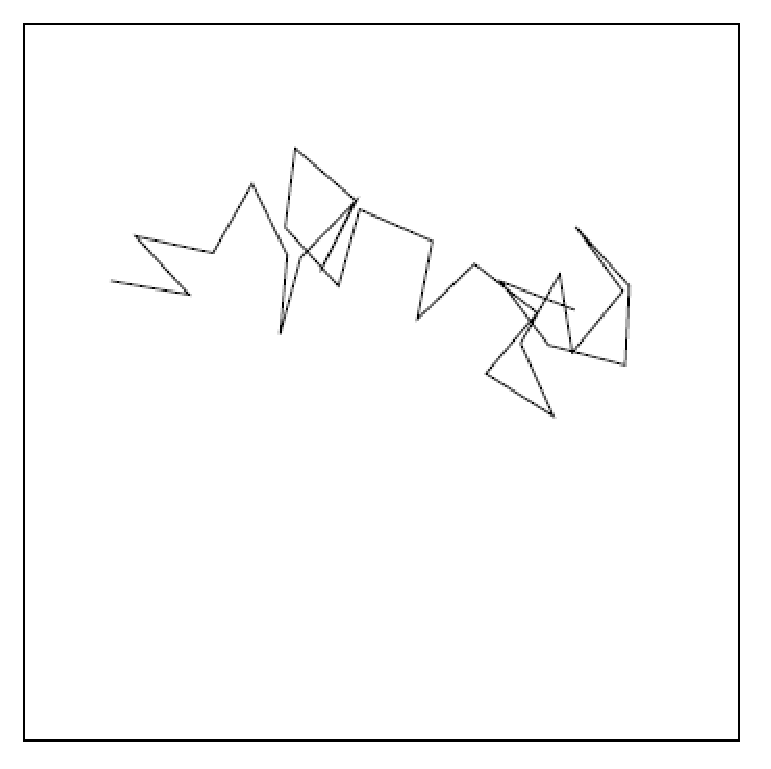
\includegraphics[scale=0.5]{caminataAleatoria_06.eps}
	\caption{Se aprecian los pasos de la caminata, la longitud es de 31 pasos.}
\end{figure}
\end{frame}
\begin{frame}
\frametitle{Invariancia de escala}
Las caminatas aleatorias son invariantes de escala:
\\
\bigskip
\begin{center}
\textcolor{blue}{Se ven iguales en todas las escalas}
\end{center}
\pause
Las caminatas aleatorias tienen una dimensión fractal $D = 2$.
%checar A Random Walk Through Fractal Dimensions
\end{frame}
\section{Construir una caminata aleatoria}
\frame{\tableofcontents[currentsection, hideothersubsections]}
\subsection{El módulo \texttt{turtle}}
\begin{frame}
\frametitle{Construyamos una caminata aleatoria}
Utilizaremos un módulo llamado \textcolor{blue}{\textbf{\texttt{turtle}}} de \python.
\\
\bigskip
Es una interfaz gráficas popular para la acercar a los menores y adolescentes en la programación.
\end{frame}
\begin{frame}
\frametitle{Caminata aleatoria con \texttt{turtle}}
Imagínate una tortuga robótica comenzando en $(0, 0)$ en el plano $x-y$.
\\
\bigskip
Después de \enquote{llamar} con el módulo a una tortuga, usamos la función \funcionazul{turtle.forward($15$)}
\\
\bigskip
\pause
La tortuga se mueve $15$ píxeles en pantalla en dirección hacia adelante, dibujando una línea a medida que se mueve.
\end{frame}
\begin{frame}
\frametitle{Caminata aleatoria con \texttt{turtle}}
Si usamos ahora la función \funcionazul{turtle.right($25$)}, ésta gira un ángulo de $25$ grados en el sentido de las manecillas del reloj.
\\
\bigskip
Con la combinación de éstos comandos y otros similares, podemos dibujar formas complejas fácilmente.
\end{frame}
\subsection*{Modelo de color HSV}
\begin{frame}
\frametitle{Algo muy breve de teoría del color}
El modelo HSV (del inglés Hue, Saturation, Value – Matiz, Saturación, Valor), también llamado HSB (Hue, Saturation, Brightness – Matiz, Saturación, Brillo), define un modelo de color en términos de sus componentes.
\end{frame}
\begin{frame}
\frametitle{El Matiz}
El matiz es el término más básico del color y denota el color de un objeto.
\\
\bigskip
Cuando decimos \enquote{azul}, \enquote{rojo} o \enquote{verde}, se habla de matices.
\end{frame}
\begin{frame}
\frametitle{La saturación}
La saturación se refiere a cómo un matiz aparece bajo ciertas condiciones de luz.
\\
\bigskip
Podemos pensar en la saturación en términos de débil vs. fuerte o matices pálidos vs. puros.     
\end{frame}
\begin{frame}
\frametitle{El valor}
El valor podría ser llamado también \enquote{claridad}.
\\
\bigskip
Se refiere a qué tan claro u oscuro es un color. Los colores claros tienen valores más altos.
\\
\bigskip
Por ejemplo, el naranja tiene un valor más alto que el azul marino. El negro tiene el menor valor de todos los colores y el blanco tiene el más alto.
\end{frame}
\begin{frame}
\frametitle{¿Para qué queremos el HSV}
Para la caminata aleatoria que elaboraremos, se va a dibujar la trayectoria con un color, para evitar que con el mismo color negro se empalmen los trazos.
\\
\bigskip
Entonces lo que haremos será decirle a la computadora que cambie el color de acuerdo a cierta instrucción, que recibirá la función \funcionazul{hsv\_to\_rgb}, que modificará el color con el modelo RGB (rojo, verde, azul), que es el que utiliza \python{}.
    


\end{frame}
\begin{frame}[plain, allowframebreaks, fragile]
\frametitle{Código con python}
\begin{lstlisting}[caption=Definición del espacio de trabajo, style=FormattedNumber, basicstyle=\linespread{1.1}\ttfamily=\small, columns=fullflexible]
import turtle
from random import randint
from colorsys import hsv_\textunderscore_to_\textunderscore_rgb

#longitud del paso
paso = 30

#numero de pasos
npasos = 2000

#cambia el valor de matiz de color
hinc = 1.0/npasos

#ancho de la linea
turtle.width(2)
\end{lstlisting}
\end{frame}
\begin{frame}[plain, allowframebreaks, fragile]
\frametitle{Código con \python}
\begin{lstlisting}[caption=Aspecto gráfico del entorno, style=FormattedNumber, basicstyle=\linespread{1.1}\ttfamily=\small, columns=fullflexible]
#frontera para la caminata
(w,h) = turtle.screensize()

#velocidad al dibujar
turtle.speed('fastest')

#establece el color del modelo (1:255)
turtle.colormode(1.0)

#pone el fondo de color negro
turtle.bgcolor('black')

#define el matiz
hue = 0.0
\end{lstlisting}
\end{frame}
\begin{frame}[plain, allowframebreaks, fragile]
\frametitle{Código con \python}
\begin{lstlisting}[caption=Definición de pasos y dirección, style=FormattedNumber, basicstyle=\linespread{1.1}\ttfamily=\small, columns=fullflexible]
for i in range(npasos):
	#proporciona el valor del angulo del paso
    turtle.setheading(randint(0,359))
    
    #cambia el color RGB del lapiz
    turtle.color(hsv_\textunderscore_to_\textunderscore_rgb(hue, 1.0, 1.0))
    
    #cambia el color
    hue += hinc
    
    #hace un paso hacia adelante
    turtle.forward(paso)
    
    #calcula la posicion de la tortuga
    (x,y) = turtle.pos()
    
    #revisa si esta dentro del cuadro
    if abs(x) > w or abs(y) > h:
    	
    	#si esta por fuera, se regresa
        turtle.backward(paso)
        
turtle.done()
\end{lstlisting}
\end{frame}
\begin{frame}
\frametitle{Tortuga-Ventana de salida}
\begin{figure}
	\centering
	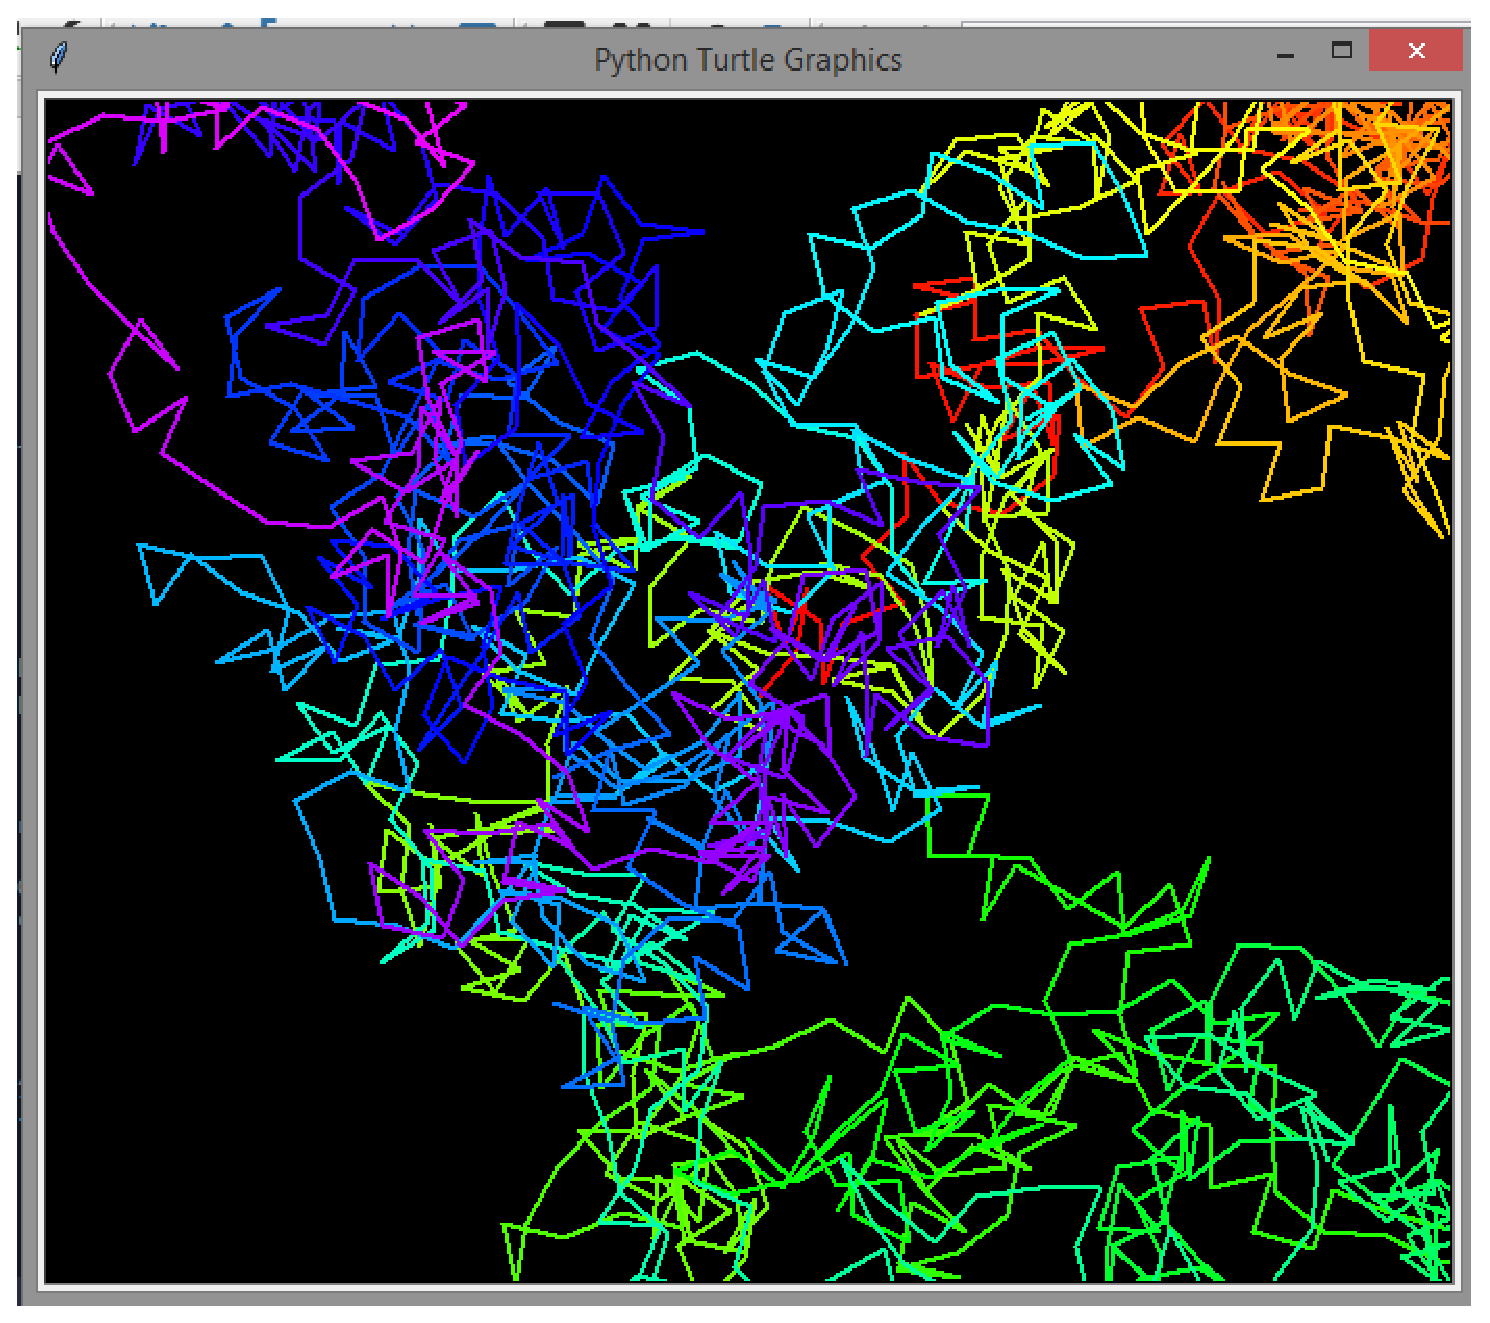
\includegraphics[scale=0.3]{Imagenes/caminataAleatoria_Python_01.eps}
\end{figure}
\end{frame}
\end{document}